\chapter{动态无向模型}
\label{chap:pgm-dynamic-undirected}

上一章用有向的动态模型描述序列：先规定状态怎样由上一时刻\emph{生成}（转移模型），再规定观测怎样由状态生成（发射模型），箭头带有明确的因果方向。但很多序列任务里，我们掌握的并不是这种“谁生成谁”的机制，而只是一些\emph{对称的相容偏好}：相邻时刻的故障标签倾向于一致（不要在正常和异常之间无意义地来回跳），同一时刻相邻设备的状态倾向于同时异常。给这类偏好硬安一个时间方向往往很别扭。更自然的做法是沿用第~\ref{chap:pgm-energy-models}章的无向能量语言，沿时间轴展开：直接为“相邻时刻状态是否相容”“同一时刻各设备状态是否相容”这些局部关系打分，再把\emph{整段}候选序列的得分放到一起共同归一化。这就是动态无向模型。

它和上一章还有一个任务层面的重要分野。上一章的HMM、状态空间模型都是\emph{生成式}的：它们为读数本身也建立分布，能生成整条序列。但在大量实际的序列标注任务里（给每个时刻判一个故障标签、做分词、词性标注），输入读数是确定已知的，我们\emph{只}关心给定读数后标签序列的条件分布，为复杂的输入建生成模型既费力又不必要。这时可以把读数固定在势函数里、只对标签序列归一化，得到动态的条件随机场。于是本章有一条和第12章平行的主线：\textbf{对全部状态联合归一化的“联合动态模型”}，与\textbf{固定输入、只对标签归一化的“条件动态模型”}。

设备先后出现两次高温报警，我们希望判断它们是否属于同一段持续故障。若几个相邻设备也同时报警，还需要考虑空间上的共同变化。上一章用状态转移和观测生成机制描述这些关系；也可以直接为“相邻时刻状态相容”“同一时刻设备状态相容”规定权重，再比较整段状态的所有候选配置。后一种做法得到沿序列展开的无向模型。

无向边不否认时间的先后，只是不把局部相容权重解释为从前一状态生成后一状态的条件概率。已知整段读数、只预测故障标签时，还可以把读数固定在势函数中，对标签序列单独归一化。下面先建立这两种归一化的共同形式，再分别讨论联合状态建模和条件序列预测，说明状态、片段与多状态耦合怎样改变推断和学习。

\section{时间相容关系的概率建模问题}
\label{sec:pgm-dynamic-undirected-common}

本节建立全章通用的两个对象：把局部相容得分沿时间拼成整段分布，以及区分联合归一化和条件归一化。二者的求和对象、训练数据和学习目标不同，这一区别贯穿后续模型。描述整段设备状态如何共同出现时，需要建立联合分布；在读数已知时预测任务标签，则建立条件分布。时间接口规定计算这些分布时必须一起保留哪些未知量。

\subsection{联合状态分布与条件输出分布}
\label{sec:pgm-dynamic-undirected-distributions}

把第$t$个位置的一组状态记为$\bm V_t$，序列长度为$T$；输入读数另记为$\bm x_{1:T}$。一个时间切片可以只有一个状态，也可以包含多个设备或多个标签。局部因子既可连接同一片内的变量，也可跨相邻片；重复同一种连接及参数，就形成时间模板。它描述随机变量沿序列的组织，不要求图结构随时间改变。

与第12章的静态无向模型一样，这里仍要先把每个时间切片、每对相邻切片的局部相容偏好打成分数，再用一个全局配分函数把整段所有可能序列的得分折算成概率；唯一的区别是现在的变量沿时间排开、配分函数要对一整条序列求和。先考虑相邻切片的作用。令$a_{\bm\theta,t}(\bm v_t)$为片内得分，$b_{\bm\theta,t}(\bm v_{t-1},\bm v_t)$为跨片得分；首尾边界偏好计入相应$a$。整段联合分布为
\begin{equation}
  \begin{aligned}
    F_{\bm\theta}(\bm v_{1:T})
      &=\sum_{t=1}^T a_{\bm\theta,t}(\bm v_t)
          +\sum_{t=2}^T b_{\bm\theta,t}
                         (\bm v_{t-1},\bm v_t),\\
    p_{\bm\theta}(\bm v_{1:T})
      &=\frac{\exp F_{\bm\theta}(\bm v_{1:T})}
                    {Z_{\bm\theta,T}}.
  \end{aligned}
  \label{eq:pgm-dynamic-undirected-joint}
\end{equation}
记$\mathcal V_t$为第$t$片状态空间，$\mu_t$为相应的计数测度或连续状态的Lebesgue测度，令$\mu=\bigotimes_{t=1}^T\mu_t$，则
\[
  Z_{\bm\theta,T}=\int_{\prod_t\mathcal V_t}
     \exp F_{\bm\theta}(\bm v_{1:T})\,\mu(\mathrm d\bm v_{1:T}).
\]
它对全部建模状态求和或积分。得分是负能量，各个指数得分是局部势，无须分别归一化；其概率语义承接第~\ref{chap:pgm-energy-models}章。有限离散空间及有限得分保证配分函数正且有限；连续状态则需要尾部可积，后面的高斯模型用正定二次能量满足这一条件。

如果读数已知、未知量是标签$\bm Y_{1:T}$，局部得分可以依赖输入，归一化只覆盖标签：
\begin{equation}
  p_{\bm\theta}(\bm y_{1:T}\mid\bm x_{1:T})
    =\frac{\exp F_{\bm\theta}(\bm y_{1:T};\bm x_{1:T})}
                  {Z_{\bm\theta,T}(\bm x_{1:T})}.
  \label{eq:pgm-dynamic-undirected-conditional}
\end{equation}
这里$Z_{\bm\theta,T}(\bm x_{1:T})$对标签的乘积状态空间求和或积分，输入固定为查询条件。输入特征可以使用已取得的过去、当前及未来读数；这不等于模型给输入规定了生成分布。若任务只能在线使用过去读数，就必须据此限制可用特征与查询信息，不能把整段输入下的预测当作在线预测。

本章先为每个有限$T$定义分布。即使每一段都复用相同局部势，截去末端后的边缘也未必等于另行归一化的短链：对末状态求和会留下一个依赖前端状态的边界权重。若要建立一致的无限随机过程，还须检查不同长度的边缘相容性。参数共享也只表示局部函数使用相同参数，不自动保证平稳性。

\subsection{时间接口与两类训练目标}
\label{sec:pgm-dynamic-undirected-targets}

在切片之间切开图，所有跨界因子共同涉及的未知变量构成时间接口。求和消息保留接口配置的权重，最大化消息保留最优配置；单标签链的接口只是一个标签，多设备耦合或高阶历史则可能需要多个变量。决定计算规模的是接口状态数及其可利用的因子分解，而不只是序列长度。连续模型若具有高斯闭合性，接口消息可以由均值、精度等有限参数表示。

模型的训练目标也随归一化对象改变。记$N$条独立记录的长度为$T_n$，完整状态记录为$\bm v^{(n)}$，完整输入输出记录为$(\bm x^{(n)},\bm y^{(n)})$。两类负对数似然分别是
\begin{equation}
  \begin{aligned}
    J_{\mathrm{joint}}(\bm\theta)
      &=\sum_{n=1}^{N}
        [\log Z_{\bm\theta,T_n}-F_{\bm\theta}(\bm v^{(n)})],\\
    J_{\mathrm{cond}}(\bm\theta)
      &=\sum_{n=1}^{N}
        [\log Z_{\bm\theta,T_n}(\bm x^{(n)})
          -F_{\bm\theta}(\bm y^{(n)};\bm x^{(n)})].
  \end{aligned}
  \label{eq:pgm-dynamic-undirected-objectives}
\end{equation}
学习在合法参数集合内最小化对应的$J$；需要正则化时另加$\lambda R(\bm\theta)$，其中$\lambda\geq0$和$R$的形式由拟合设定明确给出。数据得分鼓励实际记录，配分函数把所有候选配置纳入比较，防止仅把全部得分同时抬高。状态缺失或模型含潜变量时，实际记录对应多个完整配置，数据端必须先求和或积分再取对数。后续各模型将具体说明这两端需要什么边缘或矩，不能只用“最大似然”代替其学习过程。

\section{联合动态分布的建模与学习}
\label{sec:pgm-dynamic-undirected-joint-models}

联合模型评价的是“整段状态本身有多可能出现”，可用于补全缺失状态、计算多时刻事件概率、或生成一条状态序列。它在离散状态和连续状态下分别对应成对相容势和二次高斯能量；除了沿时间的持续性，还常要把同一时刻多个设备之间的空间耦合也加进来。联合模型评价整段状态的概率。给定部分时刻的状态后，可以补全其余位置；需要生成序列时，还要从该联合分布采样。状态取离散类别还是连续数值，会改变势函数及其计算方式；两条分支内部都要考察单设备时间链和设备间的空间作用。先建立共用的空间--时间得分，再在各状态域内展开模型与学习。

\label{sec:pgm-dynamic-undirected-spatiotemporal}
多个设备沿时间变化时，仅为每个设备建立独立链，会漏掉邻近设备同时过热的关系。令每片有$m$个状态$V_{t,i}$，固定空间邻接集合为$\mathcal E_s$。把空间关系和同一设备的时间持续性都加入得分：
\begin{equation}
  \begin{aligned}
    F(\bm v)= {}&\sum_{t,i}a_{t,i}(v_{t,i})
       +\sum_t\sum_{(i,j)\in\mathcal E_s}
                      c_{t,ij}(v_{t,i},v_{t,j})\\
       &+\sum_{t=2}^T\sum_i b_{t,i}(v_{t-1,i},v_{t,i}).
  \end{aligned}
  \label{eq:pgm-dynamic-undirected-spatiotemporal}
\end{equation}
整段联合分布仍按$e^F$归一化。

令这些局部函数由共享参数$\bm\theta$控制，当前任务的观测目标为
\begin{equation}
  \ell_{\mathrm{ST}}(\bm\theta)
     =\sum_{n=1}^{N}[F_{\bm\theta}(\bm v^{(n)})
                       -\log Z_{\bm\theta,T_n}].
  \label{eq:pgm-dynamic-undirected-spatiotemporal-objective}
\end{equation}
在线性特征设定下，学习比较经验特征和模型期望；非线性得分则比较参数梯度的相同期望差。空间势说明同一片内哪些状态相互作用，时间势说明哪些状态跨片相连；它们不要求输入测量存在有向生成关系。离散状态可以使用Ising、Potts或一般状态表，连续状态若使用总精度正定的二次能量，则得到稀疏时空高斯随机场。

空间共享参数汇总各位置的空间特征，时间共享参数汇总各设备的跨片特征，再与模型期望比较。完整设备阵列的一段轨迹构成一条训练记录；同段里的节点和时间片有依赖，样本单位仍应按数据收集机制确定。若依赖近似边缘计算梯度，优化停止还需结合推断误差检查，训练目标的小幅变化本身不足以确认模型期望已算准。

\subsection{离散状态的时间与空间相容关系}
\label{sec:pgm-dynamic-undirected-discrete-chain}

离散状态的无向时间链，本质上就是把第12章的Ising/Potts相容势沿时间轴接起来：每个时刻有一个“此刻更偏好哪个状态”的单点势，每对相邻时刻有一个“状态保持不变还是切换”的成对势。它能非常直接地表达“持续故障比频繁跳变更相容”这一偏好，而不必假设状态是被上一时刻按某个条件概率“生成”的。持续故障的相邻状态通常比频繁跳变的状态更相容。令$S_t\in\{1,\ldots,K\}$，用正势$\phi_t(k)$评价单点状态，用$\psi_t(j,k)$评价相邻状态组合，联合权重为
\begin{equation}
  w(s_{1:T})=\phi_1(s_1)
             \prod_{t=2}^T\psi_t(s_{t-1},s_t)\phi_t(s_t),
  \qquad p(s_{1:T})=\frac{w(s_{1:T})}{\sum_{u_{1:T}}w(u_{1:T})}.
  \label{eq:pgm-dynamic-undirected-chain-weight}
\end{equation}
二值状态$S_t\in\{-1,+1\}$可取得分$\sum_t h_tS_t+\sum_{t\ge2}J_tS_{t-1}S_t$，得到Ising链。$J_t>0$提高同号配置的相对权重，$h_t$则指定单点偏好。Potts链将同号奖励改为$J_t\mathbf1\{S_{t-1}=S_t\}$，支持多类别状态。链式分解限制为局部相邻作用，不能表达任意长程约束；但局部耦合已经可以产生远处变量的边缘相关。

训练这条离散链时，$\phi_t,\psi_t$或其共享参数是待估对象，状态记录本身是数据。记链的对数权重为$F_{\bm\theta}(s)=\log w_{\bm\theta}(s)$，本地目标为
\begin{equation}
  \ell_{\mathrm{chain}}(\bm\theta)
      =\sum_{n=1}^{N}
          [F_{\bm\theta}(s^{(n)})-\log Z_{\bm\theta,T_n}],
  \label{eq:pgm-dynamic-undirected-chain-objective}
\end{equation}
优化时既要增加数据配置的相对权重，也要重新计算所有配置的总权重。因此先掌握链式求和，才能得到正确的学习梯度。

一个三位置教学例子取$\phi_t=1$、同号边势为$3$、异号为$1$。两条边都同号的两种配置各有权重$9$，只有一条边同号的四种配置各为$3$，两条边都异号的两种配置各为$1$，总权重是$32$。每个位置的正类边缘仍为$1/2$，相邻同号的概率却为$3/4$。把三个位置各自拟合成概率$1/2$的独立状态，会遗漏这项持续性。

前向消息汇总以某个状态结束的前缀，后向消息汇总该状态之后的后缀。令$\alpha_1(k)=\phi_1(k)$、$\beta_T(k)=1$，递推为
\begin{equation}
  \begin{aligned}
    \alpha_t(k)&=\phi_t(k)\sum_j\alpha_{t-1}(j)\psi_t(j,k),\\
    \beta_{t-1}(j)&=\sum_k\psi_t(j,k)\phi_t(k)\beta_t(k),\\
    Z&=\sum_k\alpha_T(k),\qquad
    p(S_t=k)=\alpha_t(k)\beta_t(k)/Z.
  \end{aligned}
  \label{eq:pgm-dynamic-undirected-chain-messages}
\end{equation}
固定某个已观测状态时，将其余状态的单点势置零，再执行同样递推，所得归一化分布就是状态补全的条件分布。最大积和回溯则求整段最可能状态，不能替代边缘概率。一般稠密边势下，前向、后向或最优序列解码均需$O(TK^2)$时间。

有限正链也能改写为有向Markov链，但转移需要吸收后缀权重：
\begin{equation}
  p(S_t=k\mid S_{t-1}=j)
     =\frac{\psi_t(j,k)\phi_t(k)\beta_t(k)}{\beta_{t-1}(j)},
     \quad t\ge2.
  \label{eq:pgm-dynamic-undirected-chain-transition}
\end{equation}
在给定前一状态后，前缀与后缀被该状态分隔，上式由条件概率的比值直接得到，分母正好是分子的状态和。初始分布为$\phi_1(k)\beta_1(k)/Z$。因此无向链与有向链可以表示相同有限序列分布；直接把$\psi_t$逐行归一化，通常却会丢掉状态偏好和后缀影响。即使势共享参数，转换后的转移也可能随距末端的位置变化。

设完整训练序列的得分为$F_{\bm\theta}=\bm\theta^\top\bm G$，$\bm G$汇总所有位置的单点与相邻状态特征。单条记录的对数似然梯度是
\[
  \bm G(s_{1:T})-\mathbb E_{p_{\bm\theta}}\bm G(S_{1:T}).
\]
第一项来自观测状态，第二项由消息给出的单点及相邻状态边缘计算。重复参数接收全部位置的统计和；统计和里的各项依赖，并不是独立训练样本。若某些状态未观测，第一项还须改为给定已知状态后的特征期望。近似该后验与近似模型期望是两项不同误差，通用学习推导见第~\ref{chap:pgm-parameter-learning}章。

一次更新先由当前参数构造各位置的势，再用前向--后向求单点与边边缘，累加共享特征的模型期望，最后沿总对数似然梯度上升；若改为最小化负对数似然，梯度取反。加正则化时在同一目标中加入对应项。每轮检查目标值与所需边缘的精度，不能把固定势下的一次消息计算当成已经学得参数。

回到多个设备，令每片的离散向量为$(S_{t,1},\ldots,S_{t,m})$，将式~\eqref{eq:pgm-dynamic-undirected-spatiotemporal}中的空间势取为同片状态表，就把单设备链扩成离散时空随机场。联合似然仍由式~\eqref{eq:pgm-dynamic-undirected-spatiotemporal-objective}给出，学习期望却必须来自包含空间耦合的整张图。删去全部空间耦合，并使初始、边界及其余得分都按设备分解时，才退回独立设备链。

把一片的全部状态合并，可以形式上得到一条向量状态链，却不能因此忽略接口规模。每设备有$K$个状态时，一片已有$K^m$种配置，朴素稠密片间递推需$O(TK^{2m})$时间。利用原空间图及跨片因子进一步分解，可能降低实际计算；精确消元的主要限制是诱导宽度。若宽度过大，可按第~\ref{chap:pgm-variational}、\ref{chap:pgm-sampling}章近似所需边缘或期望，并检查实际查询的误差。

\subsection{连续状态的二次相容关系}
\label{sec:pgm-dynamic-undirected-gaussian-chain}

连续状态下，最自然的相容打分仍是二次型（和第12章GMRF一致）：既惩罚状态偏离偏好值太远，也惩罚相邻时刻状态差得太开（即偏好轨迹平滑）。二次能量的巨大好处依旧是配分函数恰好是一个高维高斯积分、可以解析处理，而不必枚举序列。温度或位移是连续量，状态还可能同时含多个坐标。对相邻差异及状态偏好使用二次评分，可以保留链结构并得到可解析的连续分布。令每片$\bm V_t\in\mathbb R^d$，把$\bm v_{1:T}$堆叠为$Td$维向量$\bm v$，取
\begin{equation}
  E(\bm v)=\tfrac12\bm v^\top\bm K\bm v-\bm h^\top\bm v,
  \quad \bm K=\bm K^\top\succ0,
  \qquad
  p(\bm v)=\mathcal N(\bm K^{-1}\bm h,\bm K^{-1}).
  \label{eq:pgm-dynamic-undirected-gaussian}
\end{equation}
$\bm h$是$Td$维线性得分参数，正定精度$\bm K$保证未归一化密度$e^{-E}$可积。只允许同片和相邻片关系时，$\bm K$是块三对角矩阵；非相邻块为零，表示给定其余状态后的条件独立。此类模型只表达单峰高斯序列分布，不能靠增加链长度产生非高斯多峰状态。

例如标量能量$E=\tfrac12av_1^2+\tfrac12q\sum_{t=2}^T(v_t-v_{t-1})^2$，$a,q>0$，先约束初始状态，再约束相邻差异。若去掉初始项，所有状态一起平移不改变能量，常数方向不受约束，不能在$\mathbb R^T$上归一化。这个例子说明平滑偏好本身并不足以定义合法联合分布。

线性高斯状态空间模型也可写成这种能量。用上一章的$\bm z_t,\bm x_t$与正定噪声协方差，将高斯初态、转移与观测的负对数相加，固定读数后的状态能量为
\begin{equation}
  \begin{aligned}
    E(\bm z;\bm x)
      &=\tfrac12(\bm z_1-\bm m_0)^\top\bm P_0^{-1}
                          (\bm z_1-\bm m_0)\\
      &\quad{}+\tfrac12\sum_{t=2}^{T}
        (\bm z_t-\bm A\bm z_{t-1})^\top\bm Q^{-1}
        (\bm z_t-\bm A\bm z_{t-1})\\
      &\quad{}+\tfrac12\sum_{t=1}^{T}
        (\bm x_t-\bm C\bm z_t)^\top\bm R^{-1}
        (\bm x_t-\bm C\bm z_t).
  \end{aligned}
  \label{eq:pgm-dynamic-undirected-lgssm-energy}
\end{equation}
这里略去与状态无关的项，只在构造状态条件分布时可以这样做；拟合生成参数时，噪声行列式等项仍必须保留。转移残差展开后只产生同片二次项和相邻交叉项，所以精度矩阵为块三对角。对$T\geq2$，下邻块为$-\bm Q^{-1}\bm A$；首块包含$\bm P_0^{-1}+\bm A^\top\bm Q^{-1}\bm A$，内部块包含$\bm Q^{-1}+\bm A^\top\bm Q^{-1}\bm A$，末块包含$\bm Q^{-1}$。固定观测再给每个对角块加$\bm C^\top\bm R^{-1}\bm C$，给线性项加$\bm C^\top\bm R^{-1}\bm x_t$；初态均值另给首个线性项加$\bm P_0^{-1}\bm m_0$。当$T=1$时只保留初态和当前观测两项。

反过来，正定高斯链可以按条件概率分解形成有向表示。这个有限链的转移参数可能随位置变化，并不自动等于某组齐次$\bm A,\bm Q$。因此Kalman平滑和高斯链消元可以计算同一个后验，而“拟合状态空间生成参数”与“拟合自由稀疏精度”仍是不同参数问题（参见第~\ref{chap:pgm-dynamic}章）。

联合均值满足$\bm K\bm m=\bm h$。记对角块为$\bm D_t$，下邻块为$\bm B_t=\bm K_{t,t-1}$，线性项分块为$\bm h_t$。从前向后消元，定义$\bm S_1=\bm D_1$、$\bm r_1=\bm h_1$，并递推
\begin{equation}
  \begin{aligned}
    \bm S_t&=\bm D_t-\bm B_t\bm S_{t-1}^{-1}\bm B_t^\top,\\
    \bm r_t&=\bm h_t-\bm B_t\bm S_{t-1}^{-1}\bm r_{t-1}.
  \end{aligned}
  \label{eq:pgm-dynamic-undirected-gaussian-elimination}
\end{equation}
$\bm S_t$是消去前面状态后留给当前片的精度，$\bm r_t$是相应线性项；正定性保证各Schur补仍正定。逆矩阵记号表示解线性方程的作用，实际可用Cholesky分解完成，不必显式求逆。末端先求$\bm m_T=\bm S_T^{-1}\bm r_T$，再反向代入
\[
  \bm m_t=\bm S_t^{-1}
       (\bm r_t-\bm B_{t+1}^\top\bm m_{t+1}).
\]
给定右端状态后，左端条件均值是这个仿射形式；对右端后验求期望，便得到整个链的均值。

若部分坐标$\bm v_O$已知，把其余坐标记为$\bm V_U$，条件精度仍为$\bm K_{UU}$，线性项变为$\bm h_U-\bm K_{UO}\bm v_O$。这由将已知值代入二次能量、收集未知坐标的项得到；对剩余链执行消元，就能计算状态补全的均值与协方差。

学习和不确定性评价还需要协方差。记$\bm C_t=\operatorname{Cov}(\bm V_t)$，由条件高斯的全协方差公式可得
\begin{equation}
  \begin{aligned}
    \bm C_T&=\bm S_T^{-1},\\
    \bm C_t&=\bm S_t^{-1}
       +\bm S_t^{-1}\bm B_{t+1}^\top\bm C_{t+1}
                          \bm B_{t+1}\bm S_t^{-1},\\
    \operatorname{Cov}(\bm V_t,\bm V_{t+1})
      &=-\bm S_t^{-1}\bm B_{t+1}^\top\bm C_{t+1}.
  \end{aligned}
  \label{eq:pgm-dynamic-undirected-gaussian-moments}
\end{equation}
单片和相邻片的矩已足以计算链式二次特征。一般稠密$d\times d$块下，这些递推需$O(Td^3)$时间和$O(Td^2)$存储；若要求全部非相邻协方差，输出本身可占$O(T^2d^2)$空间。把局部矩查询与显式生成完整协方差混为一谈，会夸大前者的成本\scite{pgm-undirected-rue2005}。

高斯闭式不仅给出均值，也使学习目标能够完整写出。对一条$D=Td$维记录，配方后有$\log Z=\tfrac D2\log(2\pi)-\tfrac12\log|\bm K|+\tfrac12\bm h^\top\bm K^{-1}\bm h$，因而要最小化
\begin{equation}
  \begin{aligned}
    J_{\mathrm G}(\bm K,\bm h;\bm v)
      &=-\tfrac12\log|\bm K|+\tfrac12\bm v^\top\bm K\bm v
        -\bm h^\top\bm v\\
      &\quad{}+\tfrac12\bm h^\top\bm K^{-1}\bm h
        +\tfrac D2\log(2\pi).
  \end{aligned}
  \label{eq:pgm-dynamic-undirected-gaussian-objective}
\end{equation}
多条记录累加对应目标；若参数跨位置共享，$\bm K,\bm h$表示由同一组局部参数组装出的矩阵和向量。学习保持正定性与指定零模式，不能任意优化每个矩阵元素。自然参数下，对$\bm h$的梯度为$\bm m-\bm v$，对对称$\bm K$的微分系数为$\tfrac12[\bm v\bm v^\top-(\bm K^{-1}+\bm m\bm m^\top)]$，其中$\bm m=\bm K^{-1}\bm h$。对合法自由参数按其进入$\bm K,\bm h$的方式应用链式法则，再沿负梯度更新；两类参数的符号由它们在能量中的正负号决定。

完整记录给出$\bm V_t$及$\bm V_t\bm V_s^\top$的样本统计量；块三对角结构只需要$s=t$或$s=t+1$的二阶项。拟合自然参数$\bm K,\bm h$时，似然梯度比较观测统计与上述递推计算的模型统计，同时保持$\bm K\succ0$和指定稀疏模式。若按状态空间的转移矩阵、噪声协方差参数化，则沿用对应模型的学习约束；不同参数化的优化性质不能混用。

状态部分缺失时，用给定已知状态后的均值与协方差形成期望统计量，再执行学习更新。潜在坐标及共享参数还可能不可唯一解释，有限样本也可能不足以得到非退化协方差估计；正则化和可识别条件需要随拟合目标说明。高斯闭合性解决的是概率与矩计算，不自动保证任意参数学习问题都唯一可解。

在设备阵列上，令式~\eqref{eq:pgm-dynamic-undirected-spatiotemporal}的单点、空间及时间得分均采用二次式，并约束合成能量的总精度正定，就得到稀疏时空高斯模型。按整片堆叠变量且只连接相邻时片时，精度仍可呈块三对角结构；同片空间边改变每个块内部的稀疏性。目标继续使用式~\eqref{eq:pgm-dynamic-undirected-gaussian-objective}，状态补全与学习仍需要均值和相应二阶矩。变化在于怎样利用稀疏结构取得这些量，而不是改用离散状态枚举。

高斯时空图即使成环，也可以利用正定精度的稀疏线性代数计算均值。消元时出现的填充决定分解成本，不能仅由原图边数推出线性复杂度。离散图上的环与高斯图上的环，因势函数的代数闭合性不同，带来的是不同计算问题。

\section{条件动态分布的建模与学习}
\label{sec:pgm-dynamic-undirected-conditional-models}

这一节转向本章的另一大类——条件动态模型：读数$\bm x$已知且固定，只对故障标签序列$\bm y$建模并在标签空间归一化，免去为输入建生成分布的负担。先从最直接的输出组织讲起，再逐步改变它：逐点标签链（线性链/高阶CRF）、把输出单位从单个标签换成片段（半Markov CRF）、同时保留多条相互耦合的标签链（多状态CRF），最后是在标签之外再引入未观测内部状态的模型。只需根据读数判断故障标签时，可以直接建立标签的条件分布。线性链先表达逐点标签的相邻关系；半Markov模型把输出改为片段；多状态链保留多个标签之间的耦合；潜状态模型则在已标注的任务输出之外增加内部解释。这些选择可以组合，下面按各自补充的职责展开。
\subsection{直接对任务输出配置评分}
\label{sec:pgm-dynamic-undirected-explicit-output}

报警标签可以逐位置给出，也可以用带边界的故障片段表示；多个设备属性还可能需要联合预测。本小节先固定这些任务输出，不额外设置输出之外的内部状态，比较输出的组织怎样改变相容得分与求和范围。标签是否全部可见，则作为每个模型训练时的数据条件另行说明。

\subsubsection{逐点标签链：线性链与高阶CRF}
\label{sec:pgm-energy-models-linear-chain}


上一章的HMM也可以在已知读数后推断状态。如果当前只关心这个条件问题，我们可以从其联合式出发固定$x$，得到
\begin{equation}
  p_{\bm\theta}(z\mid x)
   =\frac{\pi_{z_1}\prod_t b_{z_t}(x_t)
                      \prod_{t=2}^{T}a_{z_{t-1},z_t}}
          {\sum_{u_{1:T}}\pi_{u_1}\prod_t b_{u_t}(x_t)
                      \prod_{t=2}^{T}a_{u_{t-1},u_t}}.
  \label{eq:pgm-dynamic-undirected-hmm-conditional}
\end{equation}
取单点得分为发射对数、首点再加初态对数，边得分为转移对数，就得到一种链式相容评分。零概率可以通过零势或负无穷得分表示。这说明HMM后验属于带特定生成参数约束的条件链表达；它还要求发射密度及转移表各自合法。

若任务只需要给定读数后的标签，可以直接学习输入相关得分，不必同时给读数建立分布。一般CRF允许这些得分读取相互重叠的输入特征，未必能写成同结构标准HMM的归一化发射和转移。对HMM固定参数作条件化，只是同一分布的改写；最大化联合或观测似然，与直接最大化标签条件似然，使用的数据项与归一化项不同，不能因为前向算法相同就认定训练结果相同。

如果把每个时刻的标签都交给一个独立的逐点分类器（如逻辑回归），它只看当前读数、完全不管相邻标签，就会输出大量零碎、自相矛盾的结果——比如故障标签在正常/异常之间反复横跳，哪怕真实故障是一整段。要纠正这点，就得让整条标签序列\emph{联合}起来竞争概率：既奖励“当前读数支持这个标签”，也奖励“相邻标签彼此相容”。当这种相容只涉及相邻两个标签时，输出变量连起来正是一条链，这就是线性链条件随机场。逐点分类只能评价每个位置自己的标签，难以协调连续故障标签的相容性。让整条标签序列共同竞争，可以同时使用局部观测与标签关系。顺序标签只保留相邻相互作用时，输出图是一条链。\term{线性链条件随机场}（linear-chain CRF）将得分分为单点状态项与相邻转移项；序列长度为$T$、$y_t\in\{1,\ldots,K\}$时，写成
\begin{equation}
  \begin{aligned}
    f_{\bm{\theta}}(\bm{y},\bm{x})
      &=\sum_{t=1}^T a_t(y_t;\bm{x})
        +\sum_{t=2}^T b_t(y_{t-1},y_t;\bm{x}),\\
    p_{\bm{\theta}}(\bm{y}\mid\bm{x})
      &\propto e^{f_{\bm{\theta}}(\bm{y},\bm{x})}.
  \end{aligned}
  \label{eq:pgm-energy-models-chain-score}
\end{equation}
$a_t$评价输入与当前标签，$b_t$评价相邻标签组合。记$\phi_t(k)=e^{a_t(k;\bm{x})}$、$\psi_t(j,k)=e^{b_t(j,k;\bm{x})}$，暂略参数下标；首尾偏好可分别计入$a_1$、$a_T$。“转移”在这里是标签相容势，无须满足$\sum_k\psi_t(j,k)=1$，也不规定标签的因果生成顺序。

这里要学习的是产生$a_t,b_t$的参数$\bm\theta$。对完整标注记录$(\bm x^{(n)},\bm y^{(n)})$，本模型明确最小化
\begin{equation}
  J_{\mathrm{LC}}(\bm\theta)
   =\sum_{n=1}^{N}\left[
        \log Z_{\bm\theta}(\bm x^{(n)})
          -f_{\bm\theta}(\bm y^{(n)},\bm x^{(n)})\right]
       +\lambda R(\bm\theta).
  \label{eq:pgm-dynamic-undirected-linear-objective}
\end{equation}
第一项汇总所有候选标签，第二项取已标注序列的得分；其差使真实标签与其他候选作相对竞争。为计算目标和梯度，必须同时得到配分函数和模型边缘。

训练CRF需要算出“所有标签序列的得分总和”作为配分函数，标签序列有$K^T$条、不能枚举。和HMM一样，可按“末标签相同的前缀合并”做前向递推。要汇总所有标签序列，可将具有相同末标签的前缀合并。\term{前向消息}（forward message）$\alpha_t(k)$保存以$y_t=k$结束的长度$t$前缀权重总和。按前一标签分组，再乘入当前状态势和边势，得到
\begin{equation}
  \begin{aligned}
    \alpha_1(k)&=\phi_1(k),\\
    \alpha_t(k)&=\phi_t(k)
       \sum_{j=1}^K\alpha_{t-1}(j)\psi_t(j,k),
       \qquad t=2,\ldots,T,\\
    Z_{\bm{\theta}}(\bm{x})&=\sum_{k=1}^K\alpha_T(k).
  \end{aligned}
  \label{eq:pgm-energy-models-forward}
\end{equation}
每个长度$t$前缀只对应一个末标签对$(j,k)$，新增权重是旧前缀权重乘状态势及边势。分组没有遗漏或重复，结合初始消息即可归纳证明$\alpha_t$确为全部相应前缀权重之和。

单点边缘还需要当前位置右侧的证据。以$\beta_t(j)$保存固定$y_t=j$时、$t+1$至$T$的后缀权重和，排除当前位置的状态势，则
\begin{equation}
  \begin{aligned}
    \beta_T(j)&=1,\\
    \beta_t(j)&=\sum_{k=1}^K
         \psi_{t+1}(j,k)\phi_{t+1}(k)\beta_{t+1}(k),\\
    p(Y_t=k\mid\bm{x})
      &=\frac{\alpha_t(k)\beta_t(k)}{Z_{\bm{\theta}}(\bm{x})}.
  \end{aligned}
  \label{eq:pgm-energy-models-backward}
\end{equation}
相邻标签固定后，左右部分分别由前向和后向消息汇总，将边势和右端状态势接入可得
\begin{equation}
  p(Y_{t-1}=j,Y_t=k\mid\bm{x})
   =\frac{\alpha_{t-1}(j)\psi_t(j,k)
                   \phi_t(k)\beta_t(k)}
          {Z_{\bm{\theta}}(\bm{x})}.
  \label{eq:pgm-energy-models-edge-marginal}
\end{equation}
链得分的特征只涉及单点或相邻标签，因此这两类边缘足以形成全部模型期望。递推利用的是分配律下的求和消元（通用说明参见第~\ref{chap:pgm-elimination}章）。

用一个三位置的教学例子检查固定输入怎样影响标签。取$y_t\in\{-1,+1\}$，同号、异号边势仍为$3$、$1$。输入给三个位置的状态势分别为$(1,2)$、$(1,1)$、$(1,3)$，顺序为$(-1,+1)$，即首尾偏好正类、中点无单点偏好。表~\ref{tab:pgm-energy-models-chain-weights}列出全部配置，可据此核查消息、归一化及解码。

\begin{table}[htbp]
  \centering
  \begin{tabular}{crr}
    \toprule
    状态或标签配置 & 联合权重$w_0$ & 条件权重$w_{\bm{x}}$\\
    \midrule
    $(-,-,-)$ & $9$ & $9$\\
    $(-,-,+)$ & $3$ & $9$\\
    $(-,+,-)$ & $1$ & $1$\\
    $(-,+,+)$ & $3$ & $9$\\
    $(+,-,-)$ & $3$ & $6$\\
    $(+,-,+)$ & $1$ & $6$\\
    $(+,+,-)$ & $3$ & $6$\\
    $(+,+,+)$ & $9$ & $54$\\
    \midrule
    总和 & $32$ & $100$\\
    \bottomrule
  \end{tabular}
  \caption{相同边势下的两组权重。$+$、$-$代表$+1$、$-1$；条件列由联合列乘输入指定的三个状态势得到。概率应各自除以列总和，状态势本身尚不是归一化标签概率。}
  \label{tab:pgm-energy-models-chain-weights}
\end{table}

按$(-1,+1)$记录消息向量，前向结果为$\bm{\alpha}_1=(1,2)$、$\bm{\alpha}_2=(5,7)$、$\bm{\alpha}_3=(22,78)$，例如$\alpha_2(+1)=1(1\times1+2\times3)=7$。末消息总和给$Z(\bm{x})=100$。后向结果为$\bm{\beta}_3=(1,1)$、$\bm{\beta}_2=(6,10)$、$\bm{\beta}_1=(28,36)$，中点的正类边缘因此为
\[
  p(Y_2=+1\mid\bm{x})=\frac{7\times10}{100}=0.7.
\]
中点虽无局部类别偏好，仍从两侧势得到正类支持。两条边同号的概率各为$0.78$，这些边缘将在参数学习时用于计算模型的期望特征。

概率边缘累加各配置，完整序列解码则要找得分最大的配置。\term{Viterbi算法}（Viterbi algorithm）将前向求和换为最大化，保存最优前缀的前驱；以对数得分计算，可写为
\begin{equation}
  \begin{aligned}
    \delta_1(k)&=a_1(k;\bm{x}),\\
    \delta_t(k)&=a_t(k;\bm{x})
       +\max_j\{\delta_{t-1}(j)+b_t(j,k;\bm{x})\}.
  \end{aligned}
  \label{eq:pgm-energy-models-viterbi}
\end{equation}
为每个$(t,k)$记录达到最大值的$j$，从$\argmax_k\delta_T(k)$反向回溯，平局按固定标签顺序处理。数值例的$\exp[\delta_t(k)]$向量依次为$(1,2),(3,6),(9,54)$，最优序列是$(+,+,+)$，概率为$0.54$。逐点选择最大边缘标签最小化逐点错误的期望，联合解码则最大化整序列概率；本例两种选择恰好一致，并不构成一般等价。另有潜变量需先求和时，应求标签的边缘MAP，不能直接对全部变量共同取最大。

三种链递推的时间均为$O(TK^2)$。只求配分函数可以用$O(K)$消息空间；保存全部边缘消息或回溯前驱通常需$O(TK)$，全部稠密边势若预存还需$O(TK^2)$。长链要采用对数域log-sum-exp，或逐步缩放并保存尺度，避免下溢破坏归一化。训练的逐记录梯度同样反复执行前向后向，特征提取及编码器成本另计。

训练数据由成对的观测序列和标签序列组成，单条记录的条件对数似然是$f_{\bm\theta}(\bm y,\bm x)-\log Z_{\bm\theta}(\bm x)$。固定特征、线性得分$f_{\bm\theta}=\bm\theta^\top\bm F$时，其梯度是已标注序列的特征减去条件分布下的期望特征：
\[
  \nabla_{\bm\theta}\log p_{\bm\theta}(\bm y\mid\bm x)
   =\bm F(\bm y,\bm x)
       -\mathbb E_{p_{\bm\theta}(\bm Y\mid\bm x)}
                      \bm F(\bm Y,\bm x).
\]
特征只涉及单点及相邻标签，前向—后向边缘因而足以形成这项期望。三位置例子中，若观测标签为$(+,+,+)$，共享同号参数$\eta=\log3$的梯度为$2-2\times0.78=0.44$。它提高观测同号配置相对于全部候选序列的得分；两条边属于同一条训练记录，不能当作独立样本。

固定有限特征和完整标签使负对数似然为凸函数，但未正则化的可分数据可能没有有限最优参数。若$\lambda>0$且$R$是覆盖全部自由参数的正定二次函数，则有限数据上的目标具有强凸性并有唯一有限解；这项保证针对参数目标，仍需选择满足相应条件的优化算法。若用神经网络产生可训练得分，链上的精确推断仍可保留，参数目标却一般不再凸。

具体训练从合法有限参数开始，每轮为各记录计算势，用前向--后向取得$\log Z$、单点及边边缘，累加数据特征与模型期望的差，再根据最小化目标取反并加入$\lambda\nabla R$更新参数。停止条件应同时检查目标变化、梯度或优化器条件，以及独立记录上的预测。若某些标签缺失，数据端也要在相容标签配置中求和，不能再直接代入一组确定特征；这类目标一般也不继承完整标签下的凸性。

远处的输入信息可以进入$a_t$而不改变链递推，远处未知标签若直接耦合则会扩大图作用域。一阶链表达局部标签关系，不能单靠这种结构表示任意长程标签约束。与逐状态局部分类相比，CRF对整序列归一化，让不同标签序列共同竞争；相应代价是训练和概率查询都要处理完整链\scite{pgm-energy-models-sutton2012}。

线性链只让当前标签依赖\emph{相邻}标签，但有些规则天然要看更长的标签历史（比如某类标签后必须在若干步内出现配对标签）。可以让一次评分读取最近$r+1$个标签，扩大每个势的作用域；代价与高阶HMM类似——前向消息要携带最近$r$个标签的组合（$K^r$种历史），计算随$r$指数增长。也可以保留逐点标签、扩大连续标签的作用域。\term{高阶条件随机场}（higher-order CRF）让$(r+1)$个标签共同评分，写为$E=-\sum_t f_t(y_{t-r},\ldots,y_t;\bm{x})$，序列起点由固定哨兵补齐。消息须保存最近$r$个标签，共$K^r$种历史，各历史可接$K$个新值，故朴素递推耗时$O(TK^{r+1})$、滚动消息空间$O(K^r)$。历史状态只能按共同后缀接续，不必配置任意$K^r\times K^r$稠密转移。

高阶模型仍给每个位置输出一个标签，改变的是得分所读取的标签历史。记其得分为$F^{(r)}_{\bm\theta}(\bm y;\bm x)=\sum_t f_{\bm\theta,t}(y_{t-r:t};\bm x)$，学习目标为
\begin{equation}
  J_r(\bm\theta)=\sum_n
       [\log Z^{(r)}_{\bm\theta}(\bm x^{(n)})
          -F^{(r)}_{\bm\theta}(\bm y^{(n)};\bm x^{(n)})]
       +\lambda R(\bm\theta).
  \label{eq:pgm-dynamic-undirected-higher-objective}
\end{equation}
前向--后向现在返回$(r+1)$元标签团的边缘，线性特征梯度据此累计经验团特征与模型团特征之差，再更新参数。高阶HMM也使用有限历史的移位图，但它为状态与读数给出联合生成分布；这里直接拟合条件分布，目标和输入特征约束均不同。
\subsubsection{半Markov CRF：直接给候选片段评分}
\label{sec:pgm-energy-models-semi-higher}


无论是一阶还是高阶链CRF，输出单位始终是\emph{单个位置的标签}，对“这一整段故障持续了多久、区间内读数呈什么形状”这类天然属于\emph{片段}的特征，只能靠一个个相邻对间接拼凑，既不自然也难以对长度直接建模。更贴切的输出单位是“带标签的连续片段”：直接对一个候选片段（起止位置＋标签＋区间内输入形状）整体打分，再让各种合法分段共同竞争，这就是半Markov CRF。异常区间的长度与区间内温度形状，适合以片段整体评分，逐个相邻标签对难以直接表达这些特征。\term{半Markov条件随机场}（semi-Markov CRF）把带标签的连续片段作为输出单位，局部得分同时考虑起止位置、输入形状及前后片段标签。边界和标签共同参与所有合法分段的归一化。

记分段$\bm{s}=((a_\ell,b_\ell,k_\ell))_{\ell=1}^M$，要求各片段连续覆盖$1,\ldots,T$且不重叠，即$a_1=1$、$a_{\ell+1}=b_\ell+1$、$b_M=T$；长度限定为$1\leq b_\ell-a_\ell+1\leq L$。标签$k_\ell\in\{1,\ldots,K\}$，片段数$M$可以变化，起始哨兵取$k_0=0$。以$g(a,b,j,k;\bm{x})$评价前标签$j$接当前区间$[a,b]$、标签$k$的组合，分段概率为
\begin{equation}
  p_{\bm{\theta}}(\bm{s}\mid\bm{x})
   =\frac{\exp\!\left[
        \sum_{\ell=1}^M
          g(a_\ell,b_\ell,k_{\ell-1},k_\ell;\bm{x})
                    \right]}
          {Z_{\bm{\theta}}(\bm{x})}.
  \label{eq:pgm-energy-models-semi-distribution}
\end{equation}
求和候选包括所有合法边界、标签及片段数。此处允许相邻片段同标签；若任务要求将它们合并，就须从候选中排除同标签相邻片段，并在递推中禁止相应转移。

完整片段标注同时给出边界和类别，因此可以直接评价该分段的得分。参数学习最小化
\begin{equation}
  J_{\mathrm{semi}}(\bm\theta)=\sum_n
   \left[\log Z_{\bm\theta}(\bm x^{(n)})
     -\sum_{\ell=1}^{M_n}
       g_{\bm\theta}(a_\ell^{(n)},b_\ell^{(n)},k_{\ell-1}^{(n)},
                         k_\ell^{(n)};\bm x^{(n)})\right]
       +\lambda R(\bm\theta).
  \label{eq:pgm-dynamic-undirected-semi-objective}
\end{equation}
长度上限、相邻同标签是否允许和边界覆盖条件共同规定$Z$的候选集合；不能在分子与分母中采用两套不同的分段规则。下面的边界递推负责计算这些候选的总权重。

消息现在保留片段边界。令$A_t(k)$汇总覆盖前$t$个位置、末片段标签为$k$的权重，初始化$A_0(0)=1$、$A_0(k)=0$（$k>0$），并取$t>0$时$A_t(0)=0$。按末片段长度和前标签分组得到
\begin{equation}
  A_t(k)=
    \sum_{\ell=1}^{\min(L,t)}\sum_{j=0}^K
       A_{t-\ell}(j)
       e^{g(t-\ell+1,t,j,k;\bm{x})}.
  \label{eq:pgm-energy-models-semi-forward}
\end{equation}
$j=0$只用于首片段。每个前缀都有唯一的末片段长度$\ell$及前标签$j$，枚举它们不会重复计数；最终$Z(\bm{x})=\sum_{k=1}^KA_T(k)$。改用最大化并保存长度与前标签，可回溯最优分段。

取$T=3,K=1,L=2$检验边界的作用：长度$1$、$2$片段权重分别为$1$、$2$，不设其他得分。合法长度序列$(1,1,1),(1,2),(2,1)$的权重是$1,2,2$。递推得$A_1=1,A_2=3,A_3=5$，故$Z=5$，位置$1$后的边界概率为$(1+2)/5=3/5$。逐点标签全都相同，边界却未确定；长度上限只排除长度$3$的单片段，不排除三个同标签位置。

片段得分若已可常数时间读取，前向或后向计算需$O(TLK^2)$，全部边界消息需$O(TK)$空间，预存带转移的全部得分则需$O(TLK^2)$。只求$Z$可滚动保存最近$L$个边界。片段特征若要扫描内部位置，需另外计其成本；限制$L$虽减少计算，也排除了更长片段。动态规划的精确性仅针对已规定的候选集合\scite{pgm-energy-models-sarawagi2004}。

图~\ref{fig:pgm-energy-models-crf-scopes}显示两种不同扩展：片段模型改变输出单位及可选长度，高阶链增加递推保留的标签历史。它们可以组合，也可以由神经网络给局部势评分，成本仍由具体作用域及求值决定。跨任意远未知标签的势不属于上述有限记忆假设，不能直接沿用该递推。

\begin{figure}[htbp]
  \centering
  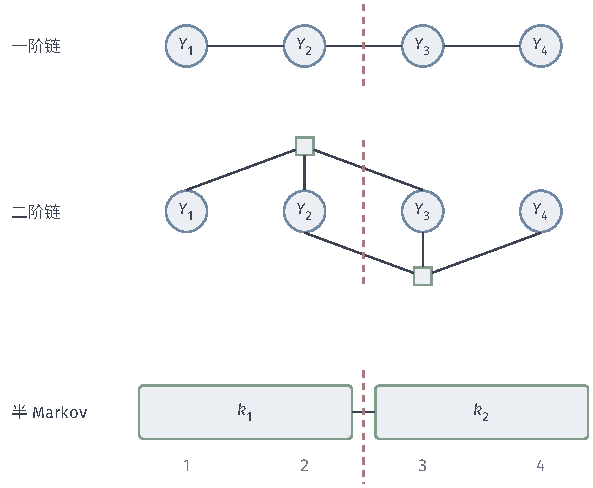
\includegraphics[width=100.404mm]{figures/09-probabilistic-graphical-models/04-models/tikz/pgm-energy-models-crf-scopes/figure.pdf}
  \caption{链、有限阶历史与片段的边界信息。一阶链在切分处保留一个标签，二阶链的跨界三元势需保留两个；半Markov模型则在片段边界汇总。图示$[1,2]$、$[3,4]$是一种候选分段，概率推断还要累加其他合法边界。}
  \label{fig:pgm-energy-models-crf-scopes}
\end{figure}

学习片段特征时还要计算它出现的边缘概率。令$B_b(k)$为边界$b$后、前标签固定为$k$的后缀权重和，取$B_T(k)=1$，按下一片段长度及标签反向汇总。前一片段标签$j$与当前区间$[a,b]$、标签$k$组成的连接，其边缘概率为
\[
  \frac{A_{a-1}(j)
           e^{g(a,b,j,k;\bm{x})}B_b(k)}
       {Z_{\bm{\theta}}(\bm{x})}.
\]
由这些边缘可计算长度、形状和转移特征的期望。完整边界及标签对应式~\eqref{eq:pgm-energy-models-semi-distribution}的直接对数似然；只有粗标签时，相容的未知分段还须在分子中求和。以最优分段替代求和会改成另一训练目标。

若$g_{\bm\theta}(a,b,j,k;\bm x)=\bm\theta^\top\bm G(a,b,j,k;\bm x)$，一条完整标注记录的梯度就是观测分段的特征和减去模型下的特征和期望。上面的连接边缘为每个候选片段提供概率权重，由此累加模型期望，再用梯度方法更新参数。完整标注、固定线性特征的负对数似然仍是凸目标；分子需要汇总未知分段时，一般失去这一保证。

与HSMM比较时，应先固定两者究竟给哪些片段配置评分。HSMM的权重来自状态边界转移、持续时间和观测生成；半Markov CRF直接根据输入给候选片段评分。只有匹配合法片段空间、起点规则与终点事件，再把相应联合权重条件化，才能得到受这些生成约束限制的条件片段模型。尤其固定观察终点的右删失与“末片段必须恰好结束”不是同一事件；共用片段动态规划并不能消除这项区别。

\subsubsection{多状态链CRF：联合保留多个输出的不确定性}
\label{sec:pgm-dynamic-undirected-factorial-crf}

到目前为止每个时刻只输出\emph{一个}标签。但我们常需要在同一时刻联合预测若干\emph{相互依赖}的输出：既要判故障\emph{类型}，又要判运行\emph{模式}，两者互相影响。若先串行地定死模式再做分类，模式一旦判错就无法被后续故障证据纠正，而且模式本身的不确定性也丢失了。正确做法是让多个标签在每个时刻都连在一起、作为一个联合输出一起归一化，保留它们之间的全部耦合。我们可能同时预测设备的故障类型与运行模式。先确定模式、再将单个预测结果交给故障分类器，会丢掉模式的不确定性，也使后续故障证据无法修正模式判断。\term{动态条件随机场}（dynamic conditional random field, DCRF）在每个时间片设置一组状态变量，并沿序列复用局部结构与参数。\term{因子条件随机场}（factorial CRF, FCRF）使用多条标签链，并增加同一时刻链间的相容关系，是一种代表构造\scite{pgm-dynamic-undirected-sutton2007}。

记第$r$条链的标签为$Y_t^{(r)}\in\{1,\ldots,K\}$，共有$R$条链，片内链间连接为$\mathcal E_c$。一种成对得分为
\begin{equation}
  \begin{aligned}
    F(\bm y;\bm x)={}&\sum_{t,r}a_t^{(r)}(y_t^{(r)};\bm x)
       +\sum_{t=2}^T\sum_r b_t^{(r)}
                (y_{t-1}^{(r)},y_t^{(r)};\bm x)\\
       &+\sum_t\sum_{(r,s)\in\mathcal E_c}
              c_t^{(r,s)}(y_t^{(r)},y_t^{(s)};\bm x).
  \end{aligned}
  \label{eq:pgm-dynamic-undirected-factorial-score}
\end{equation}
条件配分函数汇总全部标签链的联合配置。将片内耦合项去掉，且没有其他跨链作用时，分布才分解成各条独立CRF。因子HMM也组织多条状态链，但通常还为观测建立生成机制；FCRF直接评价给定输入后的标签组合，不需要给读数的相关特征规定联合分布。

以完整多链标签作为训练输出时，其具体目标是
\begin{equation}
  J_{\mathrm{FCRF}}(\bm\theta)
     =\sum_n[\log Z_{\bm\theta}(\bm x^{(n)})
                 -F_{\bm\theta}(\bm y^{(n)};\bm x^{(n)})]
       +\lambda R(\bm\theta).
  \label{eq:pgm-dynamic-undirected-factorial-objective}
\end{equation}
这里的$\bm y^{(n)}$包括全部$R$条输出链。结构选择指定哪些链内、链间得分共享参数，学习再更新这些参数；给定输入后的去耦合分解，与因子HMM中“先验链独立、后验因共同观测耦合”是两种不同条件下的陈述。

合并$R$个标签得到$K^R$种切片状态，可以精确执行链递推；把转移当作稠密表时，基线成本为$O(TK^{2R})$。原来的因子结构可能允许更有效的消元，但片内与跨片关系组成的环不能直接当成$R$条互不影响的链。推断宽度可承受时使用团树；否则用变分或环消息等方法，并核对目标边缘。消息达到固定点不自动说明边缘正确，也不保证固定点总能达到。

所有标签都完整标注、得分对参数线性时，梯度仍是观测联合特征减去条件模型期望。不同之处在于后者需要耦合图的边缘，而非分别计算各链边缘。若只标注故障类型、没有模式标签，观测似然的分子也要对相容模式求和，数据端与模型端均需推断；不能把当前最可能模式当作完整标签而保持原目标。精确完整标签目标的凸性也不能直接迁移到这种部分标注目标。

每轮训练先在整张条件图上计算所需边缘，分别累计单点、时间边和片内边特征，再按该目标更新共享参数。有缺失标签时，增加一次带已知输出约束的推断以得到数据端期望。使用近似推断时，需分别报告目标优化与边缘近似的误差；两条链各自收敛或消息达到固定点，都不能代替联合梯度的正确性。

\subsection{通过潜在内部状态解释任务输出}
\label{sec:pgm-dynamic-undirected-hidden-crf}

前面的条件模型对观测到的输出标签之间的关系直接建模，标签本身就是全部隐结构。但同样一个“故障”标签，内部往往还要经历升温、持续过热、恢复等\emph{没有被标注}的阶段；显式建模这些内部阶段，模型能更准确地刻画标签区间内读数的演化。这就需要在任务输出之外再引入一组\emph{潜在内部状态}，训练时它们不可见、要对其所有可能取值求和——与第13章HMM加隐状态、本章条件归一化结合起来。同一种故障可能经历升温、持续过热与恢复阶段，任务标签只写“故障”，没有标注这些内部阶段。多状态链允许同时描述多类状态，潜状态模型进一步把内部阶段视为未观测变量，训练时汇总其不确定性。需要先分清两种输出：给整段序列一个类别，或给每个位置一个标签。

先建立两类模型共用的学习量。用$O$表示任务输出随机变量、$o$表示给定取值；它可以是整段类别，也可以是一条标签序列。内部状态向量为$\bm H$，配置记为$\bm h$。令$\Omega(\bm x)$为预先规定且不随待优化参数改变的合法输出--内部状态配置；线性得分在该集合上写为$F_{\bm\theta}(o,\bm h;\bm x)=\bm\theta^\top\bm G(o,\bm h,\bm x)$，其中$\bm G$是固定特征向量。先给合法配置归一化，再对与$o$相容的内部状态求和，得到
\begin{equation}
  p_{\bm\theta}(o\mid\bm x)
    =\frac{\sum_{\bm h:(o,\bm h)\in\Omega(\bm x)}
                e^{F_{\bm\theta}(o,\bm h;\bm x)}}
           {\sum_{(o',\bm h)\in\Omega(\bm x)}
                e^{F_{\bm\theta}(o',\bm h;\bm x)}}.
  \label{eq:pgm-dynamic-undirected-hidden-distribution}
\end{equation}
不允许的配置概率为零。HCRF将输出具体化为类别与其内部路径，LDCRF还要求潜路径与标签映射相容；这些区别在下面的结构中明确给出。对数概率的分子、分母分别是对数求和指数，各自的导数等于相应归一化分布下的特征期望。因此共享梯度为
\begin{equation}
  \nabla_{\bm\theta}\log p_{\bm\theta}(o\mid\bm x)
    =\mathbb E_{p_{\bm\theta}(\bm H\mid o,\bm x)}
                        \bm G(o,\bm H,\bm x)
      -\mathbb E_{p_{\bm\theta}(O,\bm H\mid\bm x)}
                        \bm G(O,\bm H,\bm x).
  \label{eq:pgm-dynamic-undirected-hidden-gradient}
\end{equation}
HCRF的$o$是一个类别，LDCRF的$o$是一条标签序列。第一项在已知输出下汇总潜状态，第二项汇总所有输出与潜状态；二者对应分子与分母的对数权重导数。对于LDCRF，输出由潜状态唯一决定，第二项可直接在潜状态链上计算。

两种模型均以$J(\bm\theta)=-\sum_n\log p_{\bm\theta}(o^{(n)}\mid\bm x^{(n)})+\lambda R(\bm\theta)$训练。每轮分别计算已知输出下的内部后验、全部合法配置下的联合后验，累加两种特征期望，再取负号并加入正则梯度来最小化$J$。内部路径没有标注，因此数据端本身也需要推断；用最优内部轨迹代替求和会改变目标。参数初始化、停止条件和独立记录评价仍需明确，不应只报告一次后验计算结果。

负对数似然是两个对数求和指数项之差，通常不再凸。潜状态数量、初始化、正则化和局部最优都影响拟合，状态置换还可能保留同一观测分布。潜状态能够丰富标签内部的解释，但仅靠观测分类效果，无法把它们唯一命名为真实故障阶段。

\subsubsection{HCRF：整段类别汇总内部状态轨迹}
\label{sec:pgm-dynamic-undirected-hcrf-model}

先考虑整段序列只输出\emph{一个}类别（判断这整段是不是某种故障）的情形。类别内部可能走过不同的隐状态轨迹，分类时应把该类别下\emph{所有}可能的内部轨迹得分都累加起来，与其他类别的总得分比较，而不是先武断选一条最优轨迹再分类。若任务只给一段完整故障记录一个类别，内部状态可以描述这段记录中经历了哪些阶段。不同类别应比较其全部内部解释的总权重，而不是先选一条路径再分类。

整段类别记为$C\in\{1,\ldots,M\}$，内部状态为$H_t\in\{1,\ldots,K\}$。\term{隐状态条件随机场}（hidden-state CRF, HCRF）的一种链式构造对类别和潜状态共同评分，取
\begin{equation}
  \begin{aligned}
    F_{\bm\theta}(c,\bm h;\bm x)
      &=\eta_c+\sum_t a_{t,c}(h_t;\bm x)
                      +\sum_{t=2}^T b_{t,c}(h_{t-1},h_t;\bm x),\\
    p_{\bm\theta}(c\mid\bm x)
      &=\frac{\sum_{\bm h}\exp F_{\bm\theta}(c,\bm h;\bm x)}
        {\sum_{c'}\sum_{\bm h}\exp F_{\bm\theta}(c',\bm h;\bm x)}.
  \end{aligned}
  \label{eq:pgm-dynamic-undirected-hcrf}
\end{equation}
类别确定待比较的整体解释，潜状态链表达该类别内部的变化。同一类别的概率累加全部相容内部轨迹，不只评价最好的一条。它适合整段已经确定的分类单元，逐点分段还需另行规定输出\scite{pgm-dynamic-undirected-quattoni2007}。

对训练记录$(\bm x^{(n)},c_n)$，本模型的目标明确为
\begin{equation}
  J_{\mathrm{HCRF}}(\bm\theta)
    =-\sum_n\log\frac{\sum_{\bm h}e^{F_{\bm\theta}(c_n,\bm h;\bm x^{(n)})}}
             {\sum_{c,\bm h}e^{F_{\bm\theta}(c,\bm h;\bm x^{(n)})}}
       +\lambda R(\bm\theta).
  \label{eq:pgm-dynamic-undirected-hcrf-objective}
\end{equation}
学习时先固定真实类别计算该类链的后验边缘，再对每个候选类别求前向权重及内部边缘，以类别后验加权形成第二项期望。类别偏置、单点特征和转移特征都由这两种期望更新，所需量在当前链结构中可以精确计算。

HCRF对每个类别执行一次潜状态链的前向求和，得到类别权重，再在类别之间归一化。每类$K$个状态、稠密转移下，$M$类查询需$O(MTK^2)$时间。以最大化替代内部求和会改变类别评分：一类有多条中等权重轨迹时，其总概率可能高于另一类的单条最佳轨迹。

\subsubsection{LDCRF：逐点标签汇总各自的内部状态}
\label{sec:pgm-dynamic-undirected-ldcrf-model}

另一类任务要给\emph{每个位置}打标签（标出故障从何时开始、何时恢复），但每个标签内部又有多个未标注阶段。可以让每组潜状态对应一个任务标签、并规定潜状态唯一决定当前标签，于是既保留逐点输出，又允许同一标签内部在多个阶段之间切换；推断时把所有映射到该标签序列的潜状态轨迹求和。若故障记录需要逐位置标注，整段类别不足以表示故障何时开始与恢复。可以让每个任务标签对应一组内部阶段，并规定内部状态唯一决定当前位置的标签；这样既保持逐点输出，又允许同一标签内部继续变化。

逐点输出$Y_t\in\{1,\ldots,M\}$时，\term{潜动态条件随机场}（latent-dynamic CRF, LDCRF）可以为每个标签$k$指定非空且两两不相交的潜状态集合$\mathcal H_k$，全部潜状态组成$\mathcal H=\bigcup_k\mathcal H_k$。潜状态链$p_{\bm\theta}(\bm h\mid\bm x)$采用式~\eqref{eq:pgm-energy-models-chain-score}的单点与相邻得分，将状态空间改为$h_t\in\mathcal H$，并对全部潜状态轨迹归一化。再汇总与标签序列相容的潜状态：
\begin{equation}
  p_{\bm\theta}(\bm y\mid\bm x)
      =\sum_{\bm h:\,h_t\in\mathcal H_{y_t}\ \forall t}
                    p_{\bm\theta}(\bm h\mid\bm x).
  \label{eq:pgm-dynamic-undirected-ldcrf}
\end{equation}
每条潜状态轨迹唯一确定一条标签序列，所以这些事件不重叠，全部标签概率之和为$1$。同一标签集合内的状态切换表达内部阶段，不同集合之间的切换表达类别变化。这一构造同时保留逐点标签与标签内部的动态解释\scite{pgm-dynamic-undirected-morency2007}。

对完整逐点标签记录，本模型最小化
\begin{equation}
  J_{\mathrm{LDCRF}}(\bm\theta)
    =-\sum_n\log\sum_{\bm h:\,h_t\in\mathcal H_{y_t^{(n)}}\ \forall t}
                    p_{\bm\theta}(\bm h\mid\bm x^{(n)})
       +\lambda R(\bm\theta).
  \label{eq:pgm-dynamic-undirected-ldcrf-objective}
\end{equation}
参数是潜链的局部得分，标签对应哪些潜状态则在当前模型中预先规定。计算梯度所需的两种期望时，分别在与已知标签相容的潜链和完整潜链上求边缘，再将它们代入式~\eqref{eq:pgm-dynamic-undirected-hidden-gradient}的两项期望进行梯度更新。这不是把每条记录先分配给一条内部路径的硬分类。若任务标签也有缺失，分子还须容纳所有与已知标签相容的输出；这属于额外的数据条件。

LDCRF先计算潜状态边缘，再对集合$\mathcal H_k$求和，得到单位置标签概率。对一条已知标签序列求概率时，将不属于对应集合的状态势置零，前向求和给出相容轨迹权重，再除以不加限制的配分函数。逐点选最大标签边缘与选择概率最大的整段标签序列仍是不同查询；把最佳潜状态轨迹映射成标签，也未必得到后者。

\section{概率对象、表示关系与任务选择}
\label{sec:pgm-dynamic-undirected-comparison}

本章模型名目不少：联合的离散链、高斯链、时空随机场，条件的线性链/高阶/半Markov/多状态CRF，以及带隐状态的HCRF、LDCRF。它们其实是在同一条时间轴上对几个\emph{不同的选择}做组合：归一化对象是全部状态还是只对标签、输出单位是单点还是片段、输出是一个还是多个、要不要再设隐状态。比较时应先固定“在对哪个随机对象建模、能读到哪些信息”，再谈两种表示是否给出同一分布、学习目标是否相同。同一条时间轴可以承载状态生成、标签预测或内部阶段解释。比较模型时，需要先固定随机对象和可用信息，再判断相同分布是否有不同表示，以及任务变化是否改变了学习目标。

\subsection{相同分布、不同参数化与不同学习目标}
\label{sec:pgm-dynamic-undirected-relations}

先判断要评价什么分布。联合链和时空随机场为建模状态规定整段概率，可以补全状态或生成配置；条件模型固定读数，只比较可能的任务输出。动态有向模型通常把转移与观测生成分开，动态无向模型通过相容势组合关系，两者在有限链和高斯链中可能表示同一分布。因此，是否有箭头与是否给输入建立生成模型，是两个需要分别判断的选择。

前面的推导给出三条不同的对应：有限正离散链通过后缀权重得到有向转移；线性高斯生成因子的二次展开给出稀疏高斯能量；固定HMM观测后，发射与转移对数形成受约束的CRF势。第一条依赖所选有限长度和边界，第二条需正定性并区分状态条件化与参数拟合，第三条只建立条件分布的表示。它们都不推出自由参数集合、学习目标或跨长度的过程一致性相同。HSMM与条件片段模型的联系还必须核对末片段的终点事件。

\subsection{输出单位、标注程度与计算代价}
\label{sec:pgm-dynamic-undirected-evaluation}

输出组织和标注情况需要分别检查。输出可能是逐点标签、整段类别、片段边界或多条耦合标签；模型还可能在这些输出之外设置内部状态。另一方面，当前训练记录的任务输出可能完整，也可能部分缺失。增设内部状态决定模型要汇总哪些解释，缺失任务标签决定数据端还要汇总哪些输出，这两项变化不能混成同一个分类依据。

若输出是逐点单标签，线性链CRF提供相邻关系和精确动态规划；需要更长的有限标签历史时，可增加消息记忆。若重点是区间长度、边界与内部形状，半Markov模型直接对片段评分。二者改变不同对象：前者扩大历史作用域，后者改变候选输出的单位，不能仅按名称中的“Markov”归为同一种改进。

多个输出任务彼此依赖时，FCRF保留同片与跨片耦合，避免把前一任务的单个预测当成确定证据；代价是更大的接口或近似推断。内部阶段没有标注时，HCRF和LDCRF在输出概率中汇总潜状态，分别面向整段类别与逐点标签。它们还可以与多状态或片段结构组合，代价要由组合后的图及查询重新分析。

计算比较应区分得分求值、概率归一化、边缘查询与最优输出。单状态离散链有有限状态递推，高斯链有解析矩计算，多变量时空或多标签图则可能需要更宽的消元或近似。隐状态链仍能精确求和，但含潜状态的最优标签查询不等于对全部变量取最大，参数训练也可能失去凸性。

训练和评价都应明确记录单位及可用观测。整段分类、逐点标签错误、完整标签序列错误和片段边界误差回答不同问题；在线预测也不能使用训练或测试时尚未到来的未来读数。按记录分离训练与评价并检查实际查询，比只报告训练目标是否下降更能说明所用模型的效果。

\section{本章小结}
\label{sec:pgm-dynamic-undirected-summary}

本章把第12章的无向相容建模沿时间轴展开：不给相邻时刻规定“谁生成谁”的方向，而是用相容权重联系相邻（及同片相邻设备的）状态，再对整段候选配置共同归一化。相邻时刻的状态可以通过相容权重联系起来，再对整段配置共同归一化。单点边缘相同的模型，仍可能对持续故障给出不同联合概率；三位置离散链说明了这一差别。时间先后不强迫局部权重具有生成方向，链式与高斯式分解也可以与有向表示对应。

模型选择首先取决于需要预测或生成的对象。联合链描述状态分布，时空耦合增加同片关系；条件链预测标签，半Markov模型增加边界与片段，FCRF协调多个输出，潜状态模型汇总未标注的内部解释。它们改变的对象可以组合，归一化与查询成本则需要随接口和因子作用域重新检查。

回到报警判断，若只需已知读数下的标签，可使用条件模型；若还需状态或读数的生成预测，就要明确联合建模的变量及观测机制。无论采用哪种表示，都应分别确认分布合法、所需查询可算、训练目标可求解，以及评价使用的信息是否符合任务。

\paragraph{延展阅读}
Sutton与McCallum的教程可用于复核线性链、条件似然和消息计算；Sarawagi与Cohen的半Markov工作展开片段输出。多状态依赖可继续读Sutton等人的动态条件随机场，潜状态输出可对照Quattoni等人的HCRF与Morency等人的LDCRF。连续链和稀疏时空推断则可接到Rue与Held的高斯随机场教材，重点比较查询对象及精度矩阵结构\scite{pgm-energy-models-sutton2012,pgm-energy-models-sarawagi2004,pgm-dynamic-undirected-sutton2007,pgm-dynamic-undirected-quattoni2007,pgm-dynamic-undirected-morency2007,pgm-undirected-rue2005}。
